\chapter{Series de Fourier (Tiempo continuo)}

\section{Motivaci\'{o}n}

\textquestiondown Para que estudiamos series de Fourier? Veremos que es posible representar una se\~{n}al de dos formas diferentes, una en el dominio del tiempo y otra en el dominio de la frecuencia. En otras palabras, podemos visualizar la se\~{n}al de dos formas: una cuyo eje horizontal corresponde al tiempo, y otra cuyo eje horizontal corresponde a la frecuencia. En las dos representaciones tenemos la misma informaci\'{o}n.

La forma m\'{a}s sencilla de comenzar a trabajar en el dominio de la frecuencia es graficar los coeficientes de series de Fourier en funci\'{o}n de las frecuencias de las arm\'{o}nicas de funciones peri\'{o}dicas. En las aplicaciones de procesamiento de se\~{n}ales y electr\'{o}nica, nos interesa conocer la distribuci\'{o}n de energ\'{\i}a en funci\'{o}n de la frecuencia.

\section{Definiciones}

Recordemos que una se\~{n}al $x(t)$ es peri\'{o}dica si y s\'{o}lo si existe el per\'{\i}odo, un n\'{u}mero $T > 0$ que cumple con la condici\'{o}n
\begin{equation}
    x\left( t\right) =x\left( t+T\right),
\end{equation}
para todo valor de $t$. Como ejemplos, veamos las siguientes funciones
\begin{eqnarray}
x(t) &=&\cos \left( \omega \, t\right) = 
\cos \left(\omega \, (t+\frac{2 \, \pi}{\omega}) \right) = \cos\left(\omega \, t + 2 \, \pi\right), \\
x\left( t\right) &=& \sin\left(\omega \, t \right) = 
\sin \left(\omega \, (t+\frac{2 \, \pi}{\omega})\right)  = \sin\left(\omega \, t + 2 \, \pi\right), \\
x\left( t\right) &=&e^{j \, \omega \, t} = e^{j \, \omega \,(t+\frac{2 \, \pi}{\omega})}  = e^{j \, \omega \, t} \, e^{j \, 2 \, \pi}.
\end{eqnarray}
En estos casos $T = \frac{2 \, \pi}{\omega}$. Recordemos adem\'{a}s que $e^{j \, 2 \, \pi} = cos(2 \, \pi) + j \, sin(2 \, \pi) = 1$.



\subsection{Se\~{n}ales peri\'{o}dicas arm\'{o}nicamente relacionadas}

Podemos definir a las se\~{n}ales peri\'{o}dicas arm\'{o}nicamente relacionadas como
\begin{equation}
\phi _{k}\left( t\right) =e^{j \, k \, \omega \, t}=e^{j \, k \left( \frac{2 \, \pi }{T}\right)
t}, k=0,\pm 1,\pm 2,...
\end{equation}

\begin{equation}
\alpha _{k}\left( t\right) =\cos \left( k \, \omega \, t\right) =\cos\left( k \frac{2\pi }{T}t\right) , k=0,\pm 1,\pm 2,...
\end{equation}

\begin{equation}
\beta_{k}\left( t\right) =\sin\left( k \, \omega \, t\right) =\sin \left( k \, \frac{2 \, \pi }{T}t\right) , k=0,\pm 1,\pm 2,...
\end{equation}

Como ejemplo, veamos la figura (\ref{harmonic-cteps})

\begin{figure}
	\centering
	\includegraphics[width=0.7\linewidth]{graphics/harmonic-ct}
\caption{Funciones peri\'{o}dicas arm\'{o}nicas de tiempo continuo}
	\label{harmonic-cteps}
\end{figure}


\begin{enumerate}
\item  Cada una de estas familias de se\~{n}ales tiene una frecuencia fundamental $\omega $ y per\'{\i}odo fundamental $T.$

\item  Cada una de estas funciones arm\'{o}nicas es peri\'{o}dica con           per\'{\i}odo\textbf{\ }$\frac{T}{k},$ donde $\left| k \right| >0.$
\end{enumerate}

\section{Definici\'{o}n de serie de Fourier}

\subsection{Serie de Fourier (exponenciales imaginarias)}

\begin{itemize}

        \item Seg\'{u}n la definici\'{o}n de serie de Fourier podemos escribir
        \begin{equation}
                x\left( t\right) =
                        \sum_{k=-\infty }^{\infty }a_{k} \, e^{j \, k \, \omega \, t}=
                        \sum_{k=-\infty }^{\infty }a_{k} \, e^{j \, k \left( \frac{2 \, \pi }{T}\right) \, t},
        \end{equation}
        donde $x\left( t\right) $ es peri\'{o}dica con per\'{\i}odo $T.$

        \item   La sumatoria puede desdoblarse 
        \begin{equation}
                x\left( t\right) =
                        \sum_{k=-\infty }^{\infty }a_{k} \, e^{j \, k \, \omega \, t}=
                        a_{0}+
                        \left( \sum_{k=1}^{\infty }a_{k} \, e^{j \, k \, \omega \, t}\right) +
                        \left(\sum_{k=-\infty }^{-1}a_{k} \, e^{jk \, \omega \, t}\right) ,
        \end{equation}
        
        \item   Se cambian los valores extremos del \'{\i}ndice y la f\'{o}rmula de la sumatoria 
        \begin{equation}
                x\left( t\right) =
                        \sum_{k=-\infty }^{\infty }a_{k} \, e^{j \, k \, \omega \, t}=
                        a_{0}+
                        \left( \sum_{k=1}^{\infty }a_{k} \, e^{j \, k \, \omega \, t}\right) +
                        \left(\sum_{k=1}^{\infty }a_{-k} \, e^{-jk \, \omega \, t}\right) ,
        \end{equation}
        y se reescribe 
        \begin{equation}
                x\left( t\right) =
                        \sum_{k=-\infty }^{\infty }a_{k} \, e^{j \, k \, \omega \, t}=
                        a_{0}+
                        \left( \sum_{k=1}^{\infty }a_{k} \, e^{j \, k \, \omega \, t}+a_{-k} \, e^{-jk \, \omega \, t}\right) .
\end{equation}
        
        \item   Si $x\left( t\right) $ es una se\~{n}al real entonces es igual a su conjugada
\begin{equation}
      x\left( t\right) = \bar{x}\left( t\right) =\sum_{k=-\infty }^{\infty }\bar{a}_{k}^{ }e^{-jk \, \omega \, t}.
\end{equation}
        Reemplazando $n=-k$ tenemos 
        \begin{equation}
                x\left( t\right) =
                        \sum_{n=-\infty }^{\infty }\bar{a}_{-n} \, e^{j \, n \, \omega \, t}=
                        \sum_{k=-\infty }^{\infty }a_{k} \, e^{j \, k \, \omega \, t},
        \end{equation}
        de donde se deduce que 
        \begin{equation}
                \bar{a}_{-k} = a_{k}.
        \end{equation}

\end{itemize}

\subsection{Serie de Fourier (senos ``y'' cosenos)}

\begin{itemize}

\item La serie de Fourier definida mediante exponenciales imaginarias es
\begin{equation}
        x\left( t\right) =\sum_{k=-\infty }^{\infty }a_{k} \, e^{j \, k \, \omega \, t} =
	a_{0}+
	\left( \sum_{k=1}^{\infty }a_{k} \, e^{j \, k \, \omega \, t}+a_{-k} \, e^{-jk \, \omega \, t}\right) .
         \label{sfcuno}
\end{equation}

\item Sus coeficientes complejos son
\begin{eqnarray}
        a_{k} &=&B_{k}+jC_{k},  \label{sfcdos} \\
        a_{-k} = \bar{a_{k}} &=&B_{k}-j \, C_{k}. \label{sfctres}
\end{eqnarray}

\item Tenemos por lo tanto, reemplazando (\ref{sfcdos}) y (\ref{sfctres})  en (\ref{sfcuno}),
\begin{equation}
        x\left( t\right) =
                B_{0}+
                \left[ \sum_{k=1}^{\infty }\left(B_{k}+j \, C_{k}\right) e^{j \, k \, \omega \, t}+
                \left( B_{k}-j \, C_{k}\right) e^{-j \, k \, \omega \, t}\right].
\end{equation}

\item Reagrupando exponenciales con coeficientes $B$ y exponenciales con coeficientes $C$, tenemos
\begin{equation}
        x\left( t\right) =
                B_{0}+
                \left[ \sum_{k=1}^{\infty }B_{k}
        \left( e^{j \, k \, \omega \, t}+e^{-j \, k \, \omega \, t}\right) +j \, C_{k}\left( e^{j \, k \, \omega \, t}-e^{-jk \, \omega \, t}\right) \right].
\end{equation}

\item Multiplicando y dividiendo por $2$ y considerando que $j = -\frac{1}{j}$, obtenemos
\begin{equation}
x\left( t\right) = 
  B_{0} +
  2 \, \left[ \sum_{k=1}^{\infty}
             B_{k} \, \frac{\left(e^{j \, k \, \omega \, t}+e^{-jk \, \omega \, t}\right) }{2}-
             C_{k} \, \frac{\left( e^{j \, k \, \omega \, t}-e^{-jk \, \omega \, t}\right) }{2 \, j}
       \right].
\end{equation}

\item Finalmente, aplicando las igualdades (\ref{coseuler}) y (\ref{sineuler}), resulta
\begin{equation}
x\left( t\right) =
  B_{0}+
  2 \, \left[ \sum_{k=1}^{\infty }
             B_{k} \, \cos \left( k \, \omega \, t\right) -
             C_{k} \, \sin \left( k \, \omega \, t\right) 
       \right] .
\end{equation}

\end{itemize}

\subsection{Serie de Fourier (senos con fase)}

\begin{itemize}

\item La serie de Fourier puede escribirse como
\begin{equation}
 x\left( t\right) =
D_{0}+
\left[ \sum_{k=1}^{\infty }D_{k}\sin \left( k \, \omega \, t+\theta _{k}\right) \right] .
\end{equation}

\item Considerando la ecuaci\'{o}n (\ref{sineuler}) podemos reemplazar
\begin{equation}
\sin \left( k \, \omega \, t+\theta_{k}\right) = 
\frac{e^{j \, \left( k \, \omega \, t+\theta_{k}\right)}-e^{-j \, \left( k \, \omega \, t+\theta_{k}\right)}}{2 \, j},
\end{equation}
y obtener
\begin{equation}
x\left( t\right) =
D_{0}+
\left[ \sum_{k=1}^{\infty}
    D_{k} \, 
    \frac{e^{j \, \left( k \, \omega \, t+\theta_{k}\right)}-e^{-j \, \left( k \, \omega \, t+\theta _{k}\right)}}
    {2 j}
\right] .
\end{equation}

\item Separando las exponenciales resulta
\begin{equation}
        x\left( t\right) =
                D_{0}+
                \left[ 
                        \sum_{k=1}^{\infty}
                                D_{k} \frac{e^{j \left( k \, \omega \, t+\theta _{k}\right)}}{2 j} -
                                D_{k} \frac{e^{-j \left( k \, \omega \, t+\theta _{k}\right)}}{2 j}
                \right] .
\end{equation}

\item Finalmente resulta
\begin{equation}
        x\left( t\right) =
                D_{0}+
                \left[ 
                        \sum_{k=1}^{\infty}
                                D_{k}\frac{e^{j \, \theta_{k}}}{2 j} e^{j \, k \, \omega \, t } -
                                D_{k}\frac{e^{-j \, \theta_{k}}}{2 j} e^{-j \, k \, \omega \, t}
                \right],
\end{equation}
y por lo tanto
\begin{equation}
  A_{k} = D_{k} \frac{e^{j \, \theta_{k}}}{2 j}.
\end{equation}


\end{itemize}

\subsection{Serie de Fourier (cosenos con fase)}

De la misma forma, puede transformarse
\begin{equation}
 x\left( t\right) =E_{0}+\left[ \sum_{k=1}^{\infty }E_{k} \, \cos \left( k \, \omega \, t+\theta _{k}\right) \right] .
\end{equation}
a
\begin{equation}
        x\left( t\right) =
                E_{0}+
                \left[ 
                        \sum_{k=1}^{\infty}
                                E_{k} \, \frac{e^{j \theta_{k}}}{2} \, e^{j  k \, \omega \, t } +
                                E_{k} \, \frac{e^{-j \theta_{k}}}{2} \, e^{-j  k \, \omega \, t}
                \right] .
\end{equation}

\section{C\'{a}lculo de coeficientes de la serie de Fourier}

\begin{itemize}

        \item   Por definici\'{o}n de serie de Fourier escribimos
        \begin{equation}
                x\left( t\right) =\sum_{k=-\infty }^{\infty
                }a_{k} \, e^{j \, k \, \omega \, t}. \label{sinfs}
        \end{equation}

        \item   Multipliquemos ambos miembros por $e^{-j \, n \, \omega \, t}$,
        \begin{equation}
            x\left( t\right) e^{-j \, n \, \omega \, t}=
            \sum_{k=-\infty }^{\infty } a_{k} \, e^{j \, k \, \omega \, t} \, e^{-j \, n \, \omega \, t}.
        \end{equation}

        \item   Integremos ambos miembros
        \begin{equation}
            \int_{0}^{T}x\left( t\right) \, e^{-j \, n \, \omega \, t}dt=
            \int_{0}^{T}\sum_{k=-\infty }^{\infty }a_{k} \, e^{j \, \left( k-n\right) \, \omega \, t} \, dt.
        \end{equation}
        
        \item   Intercambiamos la integral por la sumatoria
        \begin{equation}
           \int_{0}^{T}x\left( t\right) e^{-j \, n \, \omega \, t}dt=
           \sum_{k=-\infty }^{\infty}a_{k} \, 
               \left( \int_{0}^{T}e^{j \, \left( k-n\right) \, \omega \, t} \, dt\right).
        \end{equation}

        \item   Puede probarse la siguiente igualdad
        \begin{equation}
            \int_{0}^{T}e^{j \, \left( k-n\right) \omega t}dt= 
            \left\{\begin{array}{ll}
                                T & k=n, \\ 
                                0 & k \neq n.
                   \end{array} \right.
        \end{equation}
        En efecto, cuando $k=n$
        \begin{equation}
                \int_{0}^{T}e^{j \, \left( 0 \right) \, \omega t} \, dt= 
                \int_{0}^{T} dt= T.
        \end{equation}
        En cambio, cuando $k-n = m \neq 0$, entonces
        \begin{equation}
           \int_{0}^{T}e^{j \, m \, \omega \, t} \, dt= 
           \frac{1}{j \, m \, \omega} \int_{0}^{T}e^{j \, m \, \omega \, t} (j \, m \, \omega) \, dt.
        \end{equation}
        Evaluando la integral, obtenemos finalmente
        \begin{equation}
           \int_{0}^{T}e^{j m \omega t} \, dt= 
                \frac{1}{j \, m \, \omega} (e^{j \, m \, \omega \, T} - e^{0}) = 0,
        \end{equation}
        dado que
        \begin{equation}
          \omega = \frac{2 \pi}{T},
        \end{equation}
        y por lo tanto
        \begin{equation}
          e^{j \, m \, \omega T} = e^{0} = 1.
        \end{equation}

        \item   Obtenemos as\'{\i}
        \begin{equation}
            \int_{0}^{T}x\left( t\right) e^{-j \, n \, \omega \, t} \, dt = T \, a_n.
        \end{equation}
        
        \item   Definimos la ecuaci\'{o}n de an\'{a}lisis como
        \begin{equation}
            \frac{1}{T}\int_{0}^{T}x\left( t\right) e^{-j \, n \,
              \omega \, t} \, dt = a_n. \label{anafs}
        \end{equation}
\end{itemize}

\section{Condiciones para la convergencia de las series de Fourier}

Supongamos que usamos una aproximaci\'{o}n $x_{N}(t) $ con una
cantidad finita de arm\'{o}nicas a una funci\'{o}n $x(t) $
peri\'{o}dica $T$,
\begin{equation}
x_{N}\left( t\right) =\sum_{k=-N}^{N}a_{k} \, e^{j \, k \, \omega \, t},
\end{equation}
donde $\omega = \frac{2 \, \pi}{T}$.
Sea 
\begin{equation}
e_{N}\left( t\right) =x( t) -\sum_{k=-N}^{N} \, a_{k} \, e^{j \, k \, \omega \, t},
\end{equation}
el error de aproximaci\'{o}n. Definimos entonces como medida de la magnitud
del error a la integral 
\begin{equation}
E_{N}=\int_{0}^{T} \overline{e_{N}(t)} \, e_{N}(t) \, dt.
\end{equation}

\subsection{Condici\'{o}n de la energ\'{\i}a finita}

Puede probarse que 
\begin{enumerate}
\item Una se\~{n}al $x\left( t\right) $ tiene una serie de Fourier con
coeficientes $a_{k}$ finitos si la energ\'{\i}a de la se\~{n}al en un per\'{\i}odo $T$ es acotada
\begin{equation}
\int_{0}^{T} \overline{x(t)} \, x(t) dt<\infty .
\end{equation}

\item La integral $E_{N}$ es m\'{\i}nima cuando 
\begin{equation}
a_{k}=
  \frac{1}{T}\int_{0}^{T}x(t) \, e^{-j \, k \, \frac{2 \, \pi }{T}  \, t} \, dt.
\end{equation}

\item Adem\'{a}s, la integral $E_{N}$ tiende a $0$ cuando $N$ tiende a $\infty$.

\end{enumerate}

\subsection{Condiciones de Dirichlet (alternativas)}

Una se\~{n}al $x\left( t\right) $ tiene una serie de Fourier con coeficientes $a_{k}$ finitos si
\begin{enumerate}

\item  Tiene una cantidad finita de m\'{a}ximos y m\'{\i}nimos en un per\'{\i}odo.

\item  Tiene una cantidad finita de discontinuidades acotadas en un per\'{\i}odo.

\item  Su valor absoluto es integrable sobre un per\'{\i}odo 
\begin{equation}
\int_{0}^{T}\left| x\left( t\right) \right| dt<\infty .
\end{equation}

\end{enumerate}

Bajo estas condiciones, la serie de Fourier converge a $x(t)$ para todo $t$ si $x(t)$ es continua. 
En caso de que $x(t)$ sea discontinua, la serie de Fourier converge al valor medio de 
la discontinuidad para los correspondientes valores de $t$.

\section{Propiedades de las series de Fourier}

Supongamos que tenemos tres se\~{n}ales peri\'{o}dicas $x$, $y$, $z$ 
de per\'{\i}odo $T$ que pueden ser expresadas como sumas de Fourier 
con coeficientes $a_{k}$, $b_{k}$ y $c_{k}$ respectivamente. 
Podemos resumir estas hip\'{o}tesis de la siguiente forma 
\begin{eqnarray}
x\left( t\right) &=&x\left( t+T\right) 
\begin{array}{l}
FS \\ 
\longleftrightarrow
\end{array}
a_{k},  \label{xfs} \\
y\left( t\right) &=&y\left( t+T\right) 
\begin{array}{l}
FS \\ 
\longleftrightarrow
\end{array}
b_{k}, \label{yfs} \\
z\left( t\right) &=&z\left( t+T\right) 
\begin{array}{l}
FS \\ 
\longleftrightarrow
\end{array}
c_{k}. \label{zfs}
\end{eqnarray}

\subsection{Linealidad}

Las ecuaciones de an\'{a}lisis y s\'{\i}ntesis son operaciones
lineales. Podemos expresar esta propiedad de la siguiente forma: 
si la se\~{n}al $z(t)$ es una combinaci\'{o}n lineal de las
se\~{n}ales $x(t)$ e $y(t)$, con coeficientes $u$ y $v$, 
entonces los coeficientes de $z(t)$ son una combinaci\'{o}n lineal 
de los coeficientes correspondientes a $x(t)$ e $y(t)$, 
con coeficientes $u$ y $v$
\begin{equation}
z\left( t\right) = u \, x\left( t\right) + v \, y\left( t \right) 
\begin{array}{l}
FS \\ 
\longleftrightarrow
\end{array}
c_{k}=u \, a_{k} + v \, b_{k}.
\end{equation}

\begin{enumerate}

\item Para probarla, supongamos que se cumple la igualdad
\begin{equation}
  c_{k} = \frac{1}{T} \int_{0}^{T} z(t) \, e^{-j \, \frac{2 \, \pi}{T} t} \,
  dt,
\end{equation}
donde se define $z(t) = u \, x(t) + v \, y(t)$, y por lo tanto
\begin{equation}
  c_{k} = \frac{1}{T} \int_{0}^{T} \left( u \, x(t) + v \, y(t)
  \right) \, e^{-j \, \frac{2 \, \pi}{T} t} \, dt.
\end{equation}

\item Distribuyendo la exponencial y extrayendo las constantes 
$u$ y $v$ de la integral obtenemos
\begin{equation}
  c_{k} = 
    u \, \frac{1}{T} \left( \int_{0}^{T}  x(t) \, e^{-j \, \frac{2 \, \pi}{T} \,
        t} \, dt \right) +
    v \, \frac{1}{T} \left( \int_{0}^{T}  y(t) \, e^{-j \, \frac{2 \, \pi}{T} \,
        t} \, dt \right).
\end{equation}

\item Observe que, aplicando la definici\'{o}n de la ecuaci\'{o}n de
  s\'{\i}ntesis, obtenemos
\begin{equation}
  c_{k} = u \, a_{k} + v \, b_{k},
\end{equation}
como quer\' {\i}amos demostrar.

\item De otra forma, supongamos que se cumple la igualdad
\begin{equation}
  c_{k} = u \, a_{k} + v \, b_{k}.
\end{equation}

\item Multiplicando por $e^{j k \frac{2 \pi}{T} t}$ obtenemos
\begin{equation}
  c_{k} \, e^{j \, \frac{2 \, \pi}{T} \, t} = u \, a_{k} e^{j \, \frac{2 \, \pi}{T} \,
    t} + v \, b_{k} e^{j \, \frac{2 \, \pi}{T} \, t}.
\end{equation}

\item Sumando miembro a miembro resulta
\begin{equation}
  \sum_{k=-\infty}^{\infty}  c_{k} \, e^{j \, \frac{2 \, \pi}{T} \, t} = 
    \sum_{k=-\infty}^{\infty} 
      u \, a_{k} \, e^{j \, \frac{2 \, \pi}{T} \, t} + 
      v \, b_{k} \, e^{j \, \frac{2 \, \pi}{T} \, t}.
\end{equation}

\item Reacomodando la sumatoria de la derecha obtenemos
\begin{equation}
  \sum_{k=-\infty}^{\infty}  c_{k} \, e^{j \, \frac{2 \, \pi}{T} \, t} = 
    \left( \sum_{k=-\infty}^{\infty} u \, a_{k} e^{j \, \frac{2 \, \pi}{T} \,
        t} \right) + 
    \left( \sum_{k=-\infty}^{\infty} v \, b_{k} e^{j \, \frac{2 \, \pi}{T} \,
        t} \right). 
\end{equation}

\item A continuaci\'{o}n, extraemos las constantes $u$ y $v$ como
  factores comunes de las respectivas sumatorias
\begin{equation}
  \sum_{k=-\infty}^{\infty}  c_{k} \, e^{j \, \frac{2 \, \pi}{T} \, t} = 
    u \, \left( \sum_{k=-\infty}^{\infty} a_{k} e^{j \, \frac{2 \, \pi}{T} \, t} \right) + 
    v \, \left( \sum_{k=-\infty}^{\infty} b_{k} e^{j \, \frac{2 \, \pi}{T} \, t} \right). \label{linfs}
\end{equation}

\item Observando la ecuaci\'{o}n (\ref{linfs}) y las hip\'{o}tesis
  (\ref{xfs}), (\ref{yfs}) y (\ref{zfs}) , es inmediato ver que hemos
  obtenido que 
\begin{equation}
z(t) = u \, x(t) + v \, y(t).
\end{equation}

\end{enumerate}

\subsection{Desplazamiento en el tiempo}

\begin{enumerate}

\item Queremos calcular la serie de Fourier de $y(t)$ definida como
\begin{equation}
y\left( t\right) =x\left( t-t_{0}\right),
\end{equation}
conociendo la serie de Fourier de $x(t)$. Por lo tanto, probaremos que
se cumple la siguiente relaci\'{o}n
\begin{equation}
y\left( t\right) = x(t - t_{0}) = 
\begin{array}{l}
FS \\ 
\longleftrightarrow
\end{array}
b_{k}=e^{-jk \, \omega \, t_{0}} \, a_{k}.
\end{equation}

\item En efecto, aplicando la ecuaci\'{o}n de an\'{a}lisis tenemos la igualdad
\begin{equation}
b_{k}= \frac{1}{T} \, \int_{0}^{T}x\left( t-t_{0}\right) \,
e^{-jk \, \omega \, t} \, dt.
\end{equation}

\item Cambiemos la variable temporal
\begin{equation}
\tau =t-t_{0},
\end{equation}
y, extrayendo factor com\'{u}n, obtenemos la igualdad
\begin{equation}
b_{k} =e^{-j \, k \, \omega \, t_{0}} \, \frac{1}{T}\int_{0}^{T}x\left(
  \tau\right) \, e^{-j \, k \omega \tau } \, d\tau,
\end{equation}
equivalente a
\begin{equation}
b_{k} = e^{-j \, k \, \omega \, t_{0}} \, a_{k}.
\end{equation}
\end{enumerate}

\subsection{Inversi\'{o}n temporal}

\begin{enumerate}

\item Definiendo la funci\'{o}n 
\begin{equation}
y\left( t\right) =x\left( -t\right) ,
\end{equation}
podemos obtener su serie de Fourier con la siguiente relaci\'{o}n
\begin{equation}
y\left( t\right) 
\begin{array}{l}
FS \\ 
\longleftrightarrow
\end{array}
b_{k}=a_{-k},
\end{equation}

\item Consideremos la ecuaci\'{o}n de s\'{\i}ntesis con el tiempo
  invertido
\begin{equation}
y(t) = x\left( -t\right) =
\sum_{k=-\infty }^{\infty }a_{k} \, e^{-j \, k \, \omega \, t}.
\end{equation}

\item Haciendo el cambio de variable $k = -m$, obtenemos la
  ecuaci\'{o}n de s\'{\i}ntesis para $x(-t)$, 
\begin{equation}
y(t) = x\left( -t\right) =
\sum_{m=-\infty }^{\infty }a_{-m} \, e^{j \, m \, \omega \, t}.
\end{equation}
de donde se puede deducir que los coeficientes de $y(t)$ deben ser $b_{k} = a_{-k}$.

\end{enumerate}

\subsection{Escalado temporal}

\begin{enumerate}
\item Con el cambio de variables $t = \alpha \, \tau$, obtenemos una serie de
Fourier con los mismos coeficientes pero de distinta frecuencia
fundamental, como podemos ver a continuaci\'{o}n
\begin{equation}
x\left( \alpha  \, \tau \right) =
\sum_{k=-\infty }^{\infty}a_{k} \, e^{j \, k \, \omega \, \alpha \, \tau}.
\end{equation}

\item La nueva frecuencia es $\omega_{0} = \omega \, \alpha$.

\item El nuevo per\'{\i}odo es $T_{0} = \frac{T}{\alpha}$.
\end{enumerate}

\subsection{Multiplicaci\'{o}n}

\begin{enumerate}
\item Probaremos que el producto de dos funciones $x(t)$ e $y(t)$
  peri\'{o}dicas $T$ es peri\'{o}dico $T$ y sus coeficientes de
  Fourier se obtienen mediante una convoluci\'{o}n de las secuencias
  $a_{k}$ y $b_{k}$ (los coeficientes de $x(t)$ e $y(t)$)
\begin{equation}
z\left( t\right) =
x\left( t\right) y\left( t\right) \begin{array}{l}
FS \\ 
\longleftrightarrow
\end{array}
\left( c_{k}=\sum_{l=-\infty }^{\infty } a_{l} \, b_{k-l}\right).
\end{equation}

\item Sea 
\begin{equation}
z(t) = \sum_{k = -\infty}^{\infty} c_{k} \, e^{j \, k \, \frac{2 \, \pi}{T}  \, t} 
= x(t) \, y(t) = 
\left( \sum_{p = -\infty}^{\infty} a_{p} \, e^{j \, p \, \frac{2
      \,\pi}{T} \, t} \right) \, 
\left( \sum_{q = -\infty}^{\infty} b_{q} \, e^{j \, q \, \frac{2 \,
      \pi}{T} \, t} \right).
\end{equation}

\item Podemos escribir
\begin{equation}
z(t) = \sum_{k = -\infty}^{\infty} c_{k} \, e^{j \, k \, \frac{2 \,
    \pi}{T}  \, t} = 
 \sum_{p = -\infty}^{\infty} \sum_{q = -\infty}^{\infty} a_{p}
  \, b_{q} \, e^{j \, (p + q) \, \frac{2 \,\pi}{T} \, t}.
\end{equation}

\item Finalmente, con el cambio de variable $k = p + q$, y $q = k -
  p$, obtenemos
\begin{equation}
z(t) = \sum_{k = -\infty}^{\infty} c_{k} \, e^{j \, k \, \frac{2 \, \pi}{T}  \, t} = 
\sum_{k = -\infty}^{\infty} \left( \sum_{p = -\infty}^{\infty} a_{p}
  \, b_{k-p} \right) \, e^{j \, k \, \frac{2 \,\pi}{T} \, t}. \label{prodfs}
\end{equation}

\item Observando la ecuaci\'{o}n (\ref{prodfs}) podemos deducir que 
\begin{equation}
c_{k} = \sum_{p = -\infty}^{\infty} a_{p} \, b_{k-p},
\end{equation}
como quer\'{\i}amos demostrar.
\end{enumerate}

\subsection{Conjugaci\'{o}n y simetr\'{\i}a de la conjugaci\'{o}n}

\begin{enumerate}
\item Dada una funci\'{o}n peri\'{o}dica real
\begin{equation}
x\left( t\right) 
\begin{array}{l}
FS \\ 
\longleftrightarrow
\end{array}
a_{k},
\end{equation}
su conjugada est\'{a} dada por
\begin{equation}
\overline{x(t)}
\begin{array}{l}
FS \\ 
\longleftrightarrow
\end{array}
\overline{a_{-k}}.
\end{equation}

\item Si $x(t)$ es real, debe ser $\overline{x(t)} - x(t) = 0$. Por lo
  tanto 
\begin{equation}
\left(\overline{\sum_{k=-\infty}^{\infty} a_{k} \, e^{j \, k \frac{2 \,
      \pi}{T} \, t}} \right) 
-
\left(\sum_{k=-\infty}^{\infty} a_{k} \, e^{j \, k \frac{2 \,
      \pi}{T} \, t} \right) = 0.
\end{equation}

\item Distribuyendo la conjugaci\'{o}n respecto a la sumatoria,
  resulta
\begin{equation}
\left( \sum_{k=-\infty}^{\infty} \overline{a_{k} \, e^{j \, k \frac{2 \,
      \pi}{T} \, t}} \right) 
-
\left(\sum_{k=-\infty}^{\infty} a_{k} \, e^{j \, k \frac{2 \,
      \pi}{T} \, t} \right) = 0.
\end{equation}

\item Tambi\'{e}n, distribuyendo la conjugaci\'{o}n respecto al producto,
  resulta
\begin{equation}
\left( \sum_{k=-\infty}^{\infty} \overline{a_{k}} \, e^{-j \, k \frac{2 \,
      \pi}{T} \, t} \right) 
-
\left(\sum_{k=-\infty}^{\infty} a_{k} \, e^{j \, k \frac{2 \,
      \pi}{T} \, t} \right) = 0.
\end{equation}

\item Agrupando potencias iguales de $e$ resulta
\begin{equation}
\sum_{k=-\infty}^{\infty} \left( \overline{a_{-k}} - a_{k} \right) \, e^{j \, k \frac{2 \,
      \pi}{T} \, t} = 0,
\end{equation}
de donde podemos deducir $\overline{a_{-k}} = a_{k}$.

\end{enumerate}

\subsection{Funciones pares}

\begin{enumerate}

\item Si $x(t)$ es una funci\'{o}n par, entonces debe ser $x(-t) = x(t)$.

\item Desarrollando $x(t) = -x(t)$ como igualdad de series obtenemos 
\begin{equation}\sum_{k=-\infty}^{\infty} a_{k} \, e^{j \, k \,
    \omega \, t} = \sum_{k=-\infty}^{\infty} a_{k} \, e^{-j \, k \,
    \omega \, t}.
\end{equation}

\item Podemos reagrupar todo en una sumatoria
\begin{equation}
  \sum_{k=-\infty}^{\infty} \left(a_{k} - a_{-k}\right)\, 
e^{j \, k \, \omega \, t} = 0.
\end{equation}

\item Como las funciones exponenciales $e^{j \, k \, \omega \, t}$
  son distintas de $0$ para todo $t$, se desprende que 
  los coeficientes deben verificar $a_{k} - a_{-k} = 0$, 
  y por lo tanto $a_{k} = a_{-k}$.

\item Si $x(t)$ es una funci\'{o}n real, $a_{-k}$ es un n\'{u}mero complejo conjugado de $a_{k}$.
Por lo tanto, la condici\'{o}n $a_{k} = a_{-k}$ implica que la parte imaginaria de $a_{k}$ es nula.
\end{enumerate}

\subsection{Funciones impares}

\begin{enumerate}

\item Si $x(t)$ es una funci\'{o}n impar, entonces debe ser $x(t) = -x(-t)$.

\item Desarrollando $x(t) = -x(-t)$ como igualdad de series obtenemos 
\begin{equation}
   \sum_{k=-\infty}^{\infty} a_{k} \, e^{j \, k \,
    \omega \, t} = -\sum_{k=-\infty}^{\infty} a_{k} \, e^{-j \, k \,
    \omega \, t}.
\end{equation}

\item Podemos reagrupar todo en una sumatoria
\begin{equation}
  \sum_{k=-\infty}^{\infty} \left(a_{k} + a_{-k}\right)\, 
e^{j \, k \, \omega \, t} = 0.
\end{equation}

\item Como las funciones exponenciales $e^{j \, k \, \omega \, t}$
  son distintas de $0$ para todo $t$, se desprende que 
  los coeficientes deben verificar $a_{k} + a_{-k} = 0$,
  y por lo tanto $a_{k} = -a_{-k}$.

\item Si $x(t)$ es una funci\'{o}n real, $a_{-k}$ es un n\'{u}mero complejo conjugado de $a_{k}$.
Por lo tanto, la condici\'{o}n $a_{k} = -a_{-k}$ implica que la parte real de $a_{k}$ es nula.

\end{enumerate}

\subsection{Relaci\'{o}n de Parseval}

\begin{enumerate}

\item La relaci\'{o}n de Parseval expresa que la potencia total
peri\'{o}dica de $x(t)$ equivale a la suma de la potencia promedio de
todos sus componentes arm\'{o}nicos
\begin{equation}
\frac{1}{T} \int_{T} \overline{x(t)} \, x(t) dt = 
\sum_{k=-\infty }^{\infty } \overline{a_{k}} \, a_{k}.
\end{equation}

\item Empezemos con
\begin{equation}
\frac{1}{T} \int_{T} \overline{x(t)} \, x(t) dt = 
\frac{1}{T} \sum_{p = -\infty}^{\infty} \sum_{q = -\infty}^{\infty} 
\int_{T} \overline{a_{p}} \, a_{q} \, e^{j \, \left(q - p \right) \frac{2 \pi}{T} \, t} \, dt.
\end{equation}

\item Observe que si $q \neq p$, entonces
\begin{equation}
\int_{T} \overline{a_{p}} \, a_{q} \, e^{j \, \left(q - p \right)
  \frac{2 \pi}{T} \, t} \, dt = 0,
\end{equation}
 y que si $q = p = k$, entonces
\begin{equation}
\frac{1}{T} \int_{T} \overline{a_{k}} \, a_{k} \, dt =
\overline{a_{k}} \, a_{k}.
\end{equation}

\item Por lo tanto, resulta
\begin{equation}
\frac{1}{T} \int_{T} \overline{x(t)} \, x(t) dt = 
\frac{1}{T} \sum_{p = -\infty}^{\infty} \sum_{q = -\infty}^{\infty} 
\int_{T} \overline{a_{p}} \, a_{q} \, e^{j \, \left(q - p \right)
  \frac{2 \pi}{T} \, t} \, dt = 
\sum_{k = -\infty}^{\infty} \overline{a_{k}} \, a_{k},
\end{equation}
como quer\'{\i}amos demostrar.
\end{enumerate}

\subsection{Diferenciaci\'{o}n}

Dada la se\~{n}al 
\begin{equation}
x(t) = \sum_{k=-\infty }^{\infty } a_{k} \, e^{j \, k \, \omega \, t},
\end{equation}
es inmediato demostrar
\begin{equation}
\frac{dx\left( t\right) }{dt}=\sum_{k=-\infty }^{\infty } j \, k \,
\omega \, a_{k} \, e^{j \, k \, \omega \, t}.
\end{equation}

\subsection{Integraci\'{o}n}

Dada la se\~{n}al 
\begin{equation}
x(t) = \sum_{k=-\infty }^{\infty } a_{k} \, e^{j \, k \, \omega \, t},
\end{equation}
si $a_{0}=0$, entonces es inmediato probar que
\begin{equation}
\int_{-\infty }^{t} x\left( v\right) \, dv =
\sum_{k=1}^{\infty }\left( \frac{1}{j \, k \, \omega } \, a_{k} \, e^{j
    \, k \, \omega t} \right) + \sum_{k=-\infty }^{-1}\left(
  \frac{1}{j \, k \, \omega } \, a_{k} \, e^{j \, k \, \omega \, t}\right) .
\end{equation}

\section{Ejemplos}

\subsection{Tren de pulsos \label{tren.de.pulsos}}

\begin{enumerate}

\item  Calculemos la serie de Fourier de la se\~{n}al definida por 
\begin{equation}
x_{1}\left( t\right) = x_{1}(t+T) \, \left\{ 
\begin{array}{cc}
1, & 0 < t \leq T_{1}, \\ 
0, & T_{1} < t\leq T.
\end{array}
\right.
\end{equation}

\item Consideremos la ec. (\ref{anafs}), que en este caso se escribe
\begin{equation}
T \, a_{k} = \int_{0}^{T_{1}}e^{-j \, k \, \frac{2 \, \pi }{T}t} \, dt.
\end{equation}

\begin{enumerate}
\item Para $k = 0$
\begin{equation}
T \, a_{0}=\int_{0}^{T_{1}}e^{-j \, 0 \, \frac{2 \, \pi }{T}t} \, dt = \left[ t \right]_{0}^{T_{1}} = T_{1}. 
\end{equation}
y aplicando la regla de Barrow, obtenemos finalmente
\begin{equation}
T \, a_{0}=\int_{0}^{T_{1}} 1 \, dt = \left[ t \right]_{0}^{T_{1}} = T_{1}. 
\end{equation}

\item Para $k \neq 0$
\begin{equation}
T \, a_{k}=\int_{0}^{T_{1}}e^{-j \, k \, \frac{2 \, \pi }{T}t} \, dt =
\frac{1}{-j \, k \, \frac{2 \, \pi }{T}} \int_{0}^{T_{1}} e^{-j \, k \, \frac{2 \, \pi }{T}t} \, d(-j \, k \, \frac{2 \, \pi }{T} \, t),
\end{equation}
\begin{equation}
T \, a_{k}=\int_{0}^{T_{1}}e^{-j \, k \, \frac{2 \, \pi }{T}t} \, dt =
\frac{1}{-j \, k \, \frac{2 \, \pi}{T}} \, 
\left[ e^{-j \, k \, \frac{2 \, \pi}{T} \, t} \right]_{0}^{T_{1}}.
\end{equation}
y aplicando la regla de Barrow, obtenemos finalmente
\begin{equation}
T \, a_{k} =
\frac{\left(e^{\frac{-j \, 2 \, k \, \pi \, T_{1}}{T}} - 1\right)}{\frac{- j \, 2 \, k \, \pi}{T}}.
\end{equation}
\end{enumerate}

\item Asi, podemos exponer las expresiones de los coeficientes de Fourier
\begin{equation}
\left\{
\begin{array}{ll}
k=0 \rightarrow & a_{0} = \frac{T_{1}}{T}, \\ 
\\
k \neq 0 \rightarrow & a_{k}= 
\frac{T_{1}}{T} \, \frac{\left(1 - e^{-j \, k \, \frac{2 \, \pi \, T_{1}}{T}}\right)}{j \, k \, \frac{2 \, \pi \, T_{1}}{T}}.
\end{array}
\right.
\end{equation}
\end{enumerate}

A continuación vemos el código en Matlab / Octave para graficar los coeficientes de Fourier en el dominio de la frecuencia y la serie de Fourier en el dominio del tiempo.

\lstinputlisting[language=Octave]{./code/alpha.m}

\begin{figure}
	\centering
	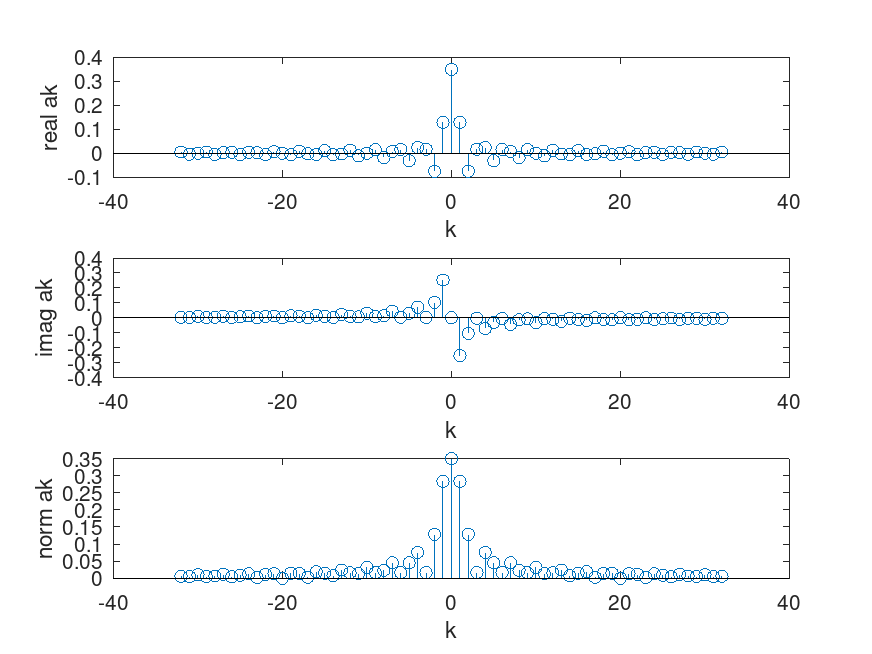
\includegraphics[width=0.7\linewidth]{code/dominio_frecuencia_alpha}
	\caption{Dominio de la frecuencia ejemplo \ref{tren.de.pulsos}}
	\label{fig:dominiofrecuenciaalpha}
\end{figure}

\begin{figure}
	\centering
	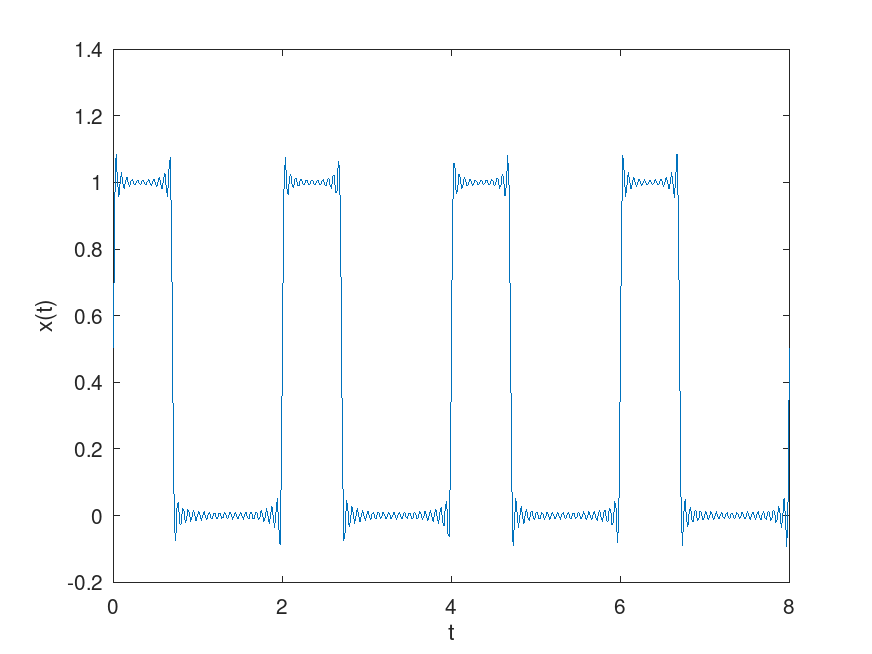
\includegraphics[width=0.7\linewidth]{code/dominio_tiempo_alpha}
	\caption{Dominio del tiempo ejemplo \ref{tren.de.pulsos}}
	\label{fig:dominiotiempoalpha}
\end{figure}

\subsection{Tren de pulsos desfasados \label{tren.de.pulsos.desplazados}}

\begin{enumerate}
\item  Calculemos la serie de Fourier de la se\~{n}al definida por 
\begin{equation}
x_{2}\left( t\right) = x_{2}\left(t + T\right) \left\{ 
\begin{array}{cc}
0, & 0 < t \leq T_{d}, \\
1, & T_{d} < t \leq T_{d} + T_{1}, \\ 
0, & T_{d} + T_{1} < t \leq T.
\end{array}
\right.
\end{equation}
Observemos que
\begin{equation}
x_{2}(t) = x_{1}(t - T_{d}),
\end{equation}
por lo que decimos que $x_{2}(t)$ es un tren de pulsos desfasados (desplazados en el tiempo).

\item Consideremos la ec. (\ref{anafs}), que en este caso se escribe como
\begin{equation}
T \, a_{k}=\int_{T_{d}}^{T_{d} + T_{1}} e^{-j \, k \, \frac{2 \, \pi }{T}t} \, dt.
\end{equation}

\item Para $k = 0$, obtenemos
\begin{equation}
T \, a_{k}=\int_{T_{d}}^{T_{d} + T_{1}} e^{-j \, 0 \, \frac{2 \, \pi }{T}t} \, dt,
\end{equation}
o, resolviendo la integral
\begin{equation}
T \, a_{k}=\int_{T_{d}}^{T_{d} + T_{1}} 1 \, dt = \left[ t \right]_{T_{d}}^{T_{d}+T_{1}} = T_{1}.
\end{equation}

\item Para $k \neq 0$, obtenemos
\begin{equation}
T \, a_{k}=\int_{T_{d}}^{T_{d} + T_{1}} \, e^{-j \, k \, \frac{2 \, \pi }{T}t} \, dt,
\end{equation}
o
\begin{equation}
T \, a_{k}=\frac{1}{-j \, k \, \frac{2 \, \pi }{T}} \int_{T_{d}}^{T_{d} + T_{1}} \, e^{-j \, k \, \frac{2 \, \pi }{T}\,t} \, d(-j \, k \, \frac{2 \, \pi }{T} \, t).
\end{equation}
Finalmente
\begin{equation}
T \, a_{k}=\frac{1}{-j \, k \, \frac{2 \, \pi }{T}}  \left[e^{-j \, k \, \frac{2 \, \pi }{T}\,t} \right]_{T_{d}}^{T_{d} + T_{1}}.
\end{equation}
Observe que podemos extraer un factor com\'{u}n de la integral
\begin{equation}
T \, a_{k}=\frac{e^{-j \, k \frac{2 \, \pi}{T} \, T_{d}}}{-j \, k \, \frac{2 \, \pi }{T}} \left[e^{-j \, k \, \frac{2 \, \pi }{T}\,t} \right]_{0}^{T_{1}},
\end{equation}
y as\'{\i} obtener finalmente
\begin{equation}
T \, a_{k}=\frac{e^{-j \, k \frac{2 \, \pi}{T} \, T_{d}}}{-j \, k \, \frac{2 \, \pi }{T}} \, 
\left(e^{-j \, k \, \frac{2 \, \pi \, T_{1}}{T}} - 1\right).
\end{equation}

\item Por lo tanto, los coeficientes de la serie de Fourier son
\begin{equation}
\left\{
\begin{array}{ll}
k=0 \rightarrow & a_{0} = \frac{T_{1}}{T}, \\ 
\\
k \neq 0 \rightarrow & a_{k}= e^{-j \, k \frac{2 \, \pi}{T} \, T_{d}} \, \frac{T_{1}}{T} \,
\frac{\left(1 - e^{-j \, k \, \frac{2 \, \pi \, T_{1}}{T}}\right)}{j \, k \, \frac{2 \, \pi \, T_{1}}{T}}.
\end{array}
\right.
\end{equation}

\item Comparando los coeficientes de $x_{1}(t)$ con los de $x_{2}(t) = x_{1}(t+T_{d})$ podemos notar
que solamente difieren en un factor $e^{-j \, k \frac{2 \, \pi}{T} \, T_{d}}$, cuya magnitud es $1$ y 
su fase es proporcional a $k$.
\end{enumerate}

\lstinputlisting[language=Octave]{./code/bravo.m}

\begin{figure}
	\centering
	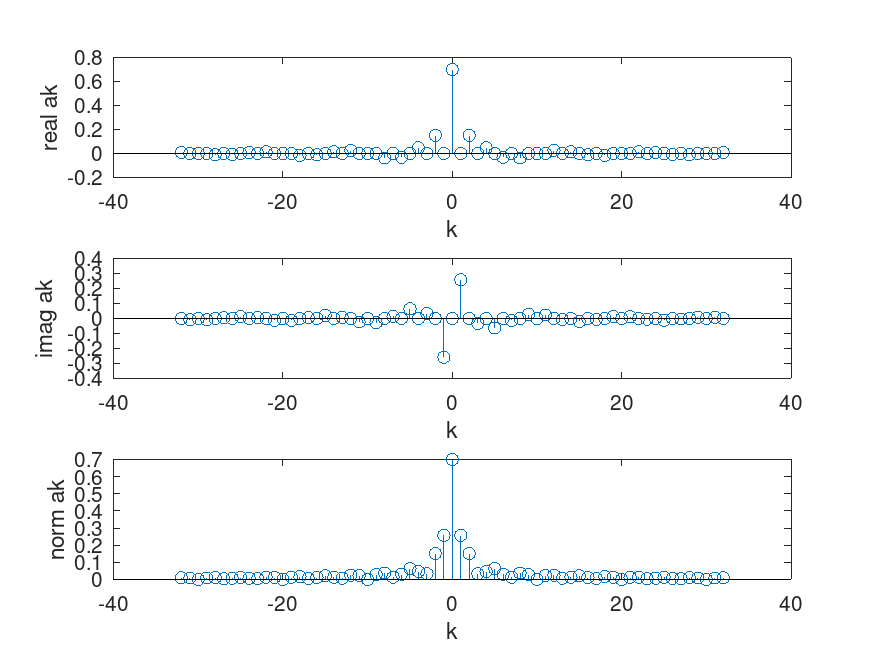
\includegraphics[width=0.7\linewidth]{code/dominio_frecuencia_bravo}
	\caption{Dominio de la frecuencia ejemplo \ref{tren.de.pulsos.desplazados}}
	\label{fig:dominiofrecuenciabravo}
\end{figure}

\begin{figure}
	\centering
	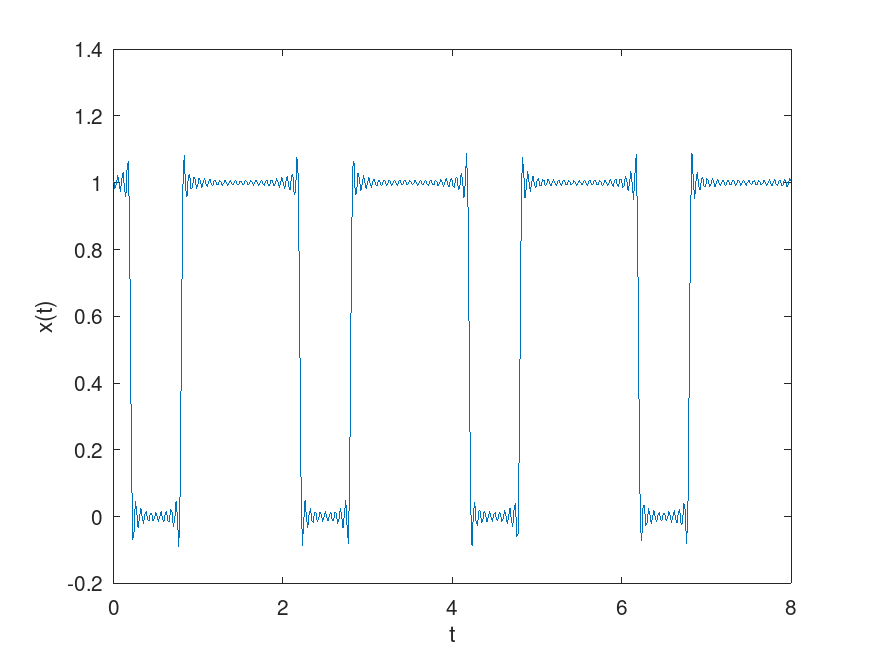
\includegraphics[width=0.7\linewidth]{code/dominio_tiempo_bravo}
	\caption{Dominio del tiempo ejemplo \ref{tren.de.pulsos.desplazados}}
	\label{fig:dominiotiempobravo}
\end{figure}

\subsection{Tren de pulsos alternados \label{tren.de.pulsos.impar}}

\begin{enumerate}
\item  Calculemos la serie de Fourier de la se\~{n}al definida por 
\begin{equation}
x_{3}\left( t\right) = x_{3}\left(t + 2 \, T \right) = 
\left\{ 
\begin{array}{cc}
-1, & -T<t \leq 0, \\ 
1, & 0 < t \leq T
\end{array}
\right.
\end{equation}

\item Entonces podemos escribir para $k = 0$,
\begin{equation}
	2 \, T \, a_{0}=
	-\int_{-T}^{0}e^{-j \, 0 \, \frac{2 \, \pi }{2 \, T} \, t} \, dt + 
	\int_{0}^{T}e^{-j \, 0 \, \frac{2 \, \pi }{2 \, T} \, t} \, dt =
	-\int_{-T}^{0} 1 \, dt + 
\int_{0}^{T} 1 \, dt = 0.
\end{equation}

\item Para $k \neq 0$ tenemos
\begin{equation}
	2 \, T \, a_{0}=
	-\int_{-T}^{0}e^{-j \, k \, \frac{2 \, \pi }{2 \, T} \, t} \, dt + 
	\int_{0}^{T}e^{-j \, k \, \frac{2 \, \pi }{2 \, T} \, t} \, dt,
\end{equation}
donde
\begin{equation}
	\int_{-T}^{0}e^{-j \, k \, \frac{2 \, \pi }{2 \, T} \, t} \, d (-j \, k \, \frac{2 \, \pi }{2 \, T})\,t = \left[e^{-j \, k \, \frac{\pi }{T} \, t}\right]_{-T}^{0} = 1 - e^{j \, k \, \frac{\pi }{T} \, T} = 1 - e^{j \, k \, \pi},
\end{equation}
y
\begin{equation}
	\int_{0}^{T}e^{-j \, k \, \frac{2 \, \pi }{2 \, T} \, t} \, d(-j \, k \, \frac{2 \, \pi }{2 \, T}) \, t = \left[e^{-j \, k \, \frac{2 \, \pi }{2 \, T} \, t}\right]_{0}^{T} = e^{-j \, k \, \frac{\pi }{T} \, T} - 1 = e^{-j \, k \, \pi} - 1.
\end{equation}

\item Por lo tanto resulta
\begin{equation}
 2 \, T \, a_{k}=
 \frac{- 1 + e^{j \, k \, \pi} + e^{-j \, k \, \pi} - 1}{-j \, k \, \frac{\pi}{T}}.
\end{equation}
\item Simplificando
\begin{equation}
	a_{k}=
	\frac{\frac{e^{j \, k \, \pi} + e^{-j \, k \, \pi}}{2} - 1}{-j \, k \, \pi}.
\end{equation}
podemos escribir
\begin{equation}
 a_{k}= j \, 
 \frac{cos(k \, \pi) - 1}{k \, \pi}.
\end{equation}
\item Observemos que cuando $k = 2 \, p$, $cos(k \, \pi) = cos(p \, 2 \, \pi) = 1$ y por lo tanto 
\begin{equation}a_{2 \, p} = 0.\end{equation}
Cuando $k = 2 \, p + 1$, entonces $cos((2 \, p + 1) \, \pi) = -1$ y 
\begin{equation}a_{2 \, p + 1} = \frac{-2 \, j}{k \, \pi}.\end{equation}

\end{enumerate}

\lstinputlisting[language=Octave]{./code/charlie.m}

\begin{figure}
	\centering
	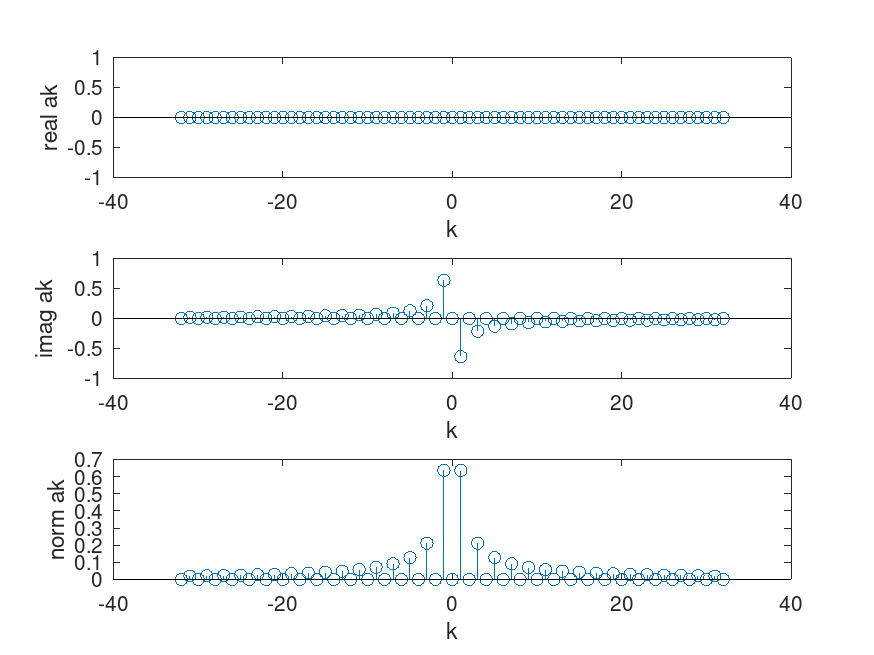
\includegraphics[width=0.7\linewidth]{code/dominio_frecuencia_charlie}
	\caption{Dominio de la frecuencia ejemplo \ref{tren.de.pulsos.impar}}
	\label{fig:dominiofrecuenciacharlie}
\end{figure}

\begin{figure}
	\centering
	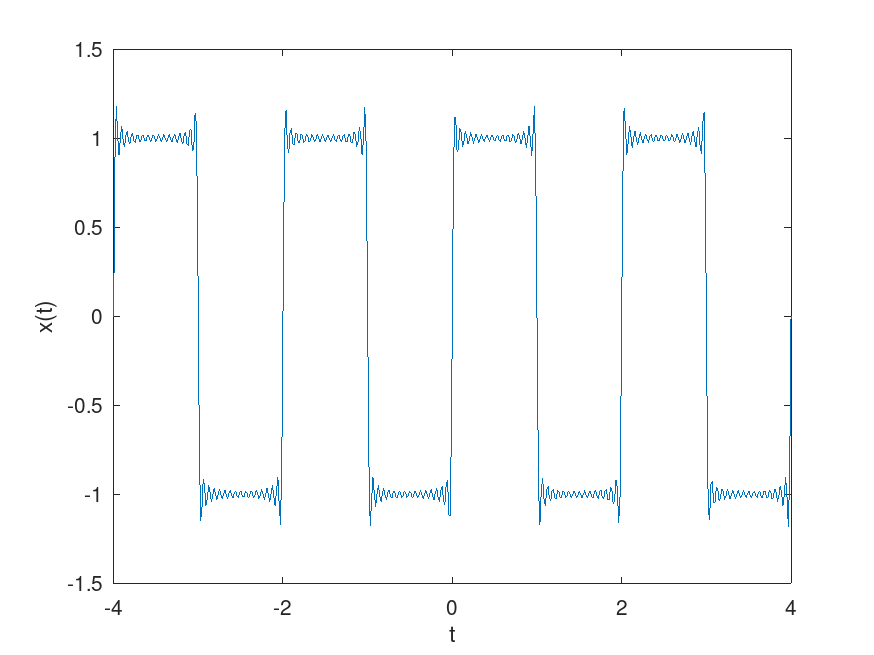
\includegraphics[width=0.7\linewidth]{code/dominio_tiempo_charlie}
	\caption{Dominio del tiempo ejemplo \ref{tren.de.pulsos.impar}}
	\label{fig:dominiotiempocharlie}
\end{figure}

\subsection{Suma de se\~{n}ales peri\'{o}dicas \label{tren.de.pulsos.suma}}

\begin{enumerate}
\item  Calculemos la serie de Fourier de la se\~{n}al definida por 
\begin{equation}
x_{4}\left( t\right) = x_{4}(t+4) \left\{
\begin{array}{cc}
1, & 0 < t \leq 1, \\
0, & 1 < t \leq 2, \\ 
-1, & 2 < t \leq 3, \\
0, & 3 < t \leq 4.
\end{array}
\right. \label{squarewave}
\end{equation}
En este caso, $x_{4}(t) = x_{1}(t) - x_{1}(t-T_{d})$, con $T = 4$, $T_{1} = 1$ y $T_{d} = 2$. Si escribimos
\begin{equation}
	x_{4}(t) = \sum_{k=-\infty}^{\infty} b_{k} \, e^{j \, k \, \frac{2 \, \pi \, t}{T}},
\end{equation}
debería ser
\begin{equation}
	b_{k} = a_{k} - a_{k} \, e^{-j \, k \, \frac{2 \, \pi \, T_{d}}{T}} = a_{k} \, (1 - e^{-j \, k \, \frac{2 \, \pi \, T_{d}}{T}}).
\end{equation}

\item Para comprobarlo, escribimos
\begin{equation}
	x_{1}(t) = \frac{1}{4} + \sum_{k=1}^{\infty} 
     \frac{1}{4} \, \frac{\left(1 - e^{-j \, k \, \frac{2 \, \pi}{4}}\right)}{j \, k \, \frac{2 \, \pi}{4}} \, e^{j \, k \, \frac{2 \, \pi \, t}{4}}
     +
     \frac{1}{4} \, \frac{\left(1 - e^{j \, k \, \frac{2 \, \pi}{4}}\right)}{-j \, k \, \frac{2 \, \pi}{4}} \, e^{-j \, k \, \frac{2 \, \pi \, t}{4}},
\end{equation}
\item También podemos escribir
\begin{equation}
	x_{1}(t-2) = \frac{1}{4} \left(1 + \sum_{k=1}^{\infty} 
	\frac{\left(1 - e^{-j \, k \, \frac{2 \, \pi}{4}}\right)}{j \, k \, \frac{2 \, \pi}{4}} \, e^{j \, k \, \frac{2 \, \pi \, (t-2)}{4}}
	+
	\frac{\left(1 - e^{j \, k \, \frac{2 \, \pi}{4}}\right)}{-j \, k \, \frac{2 \, \pi}{4}} \, e^{-j \, k \, \frac{2 \, \pi \, (t-2)}{4}}\right).
\end{equation}
y por lo tanto
\begin{equation}
	x_{1}(t-2) = \frac{1}{4} \left(1 + \sum_{k=1}^{\infty} 
	\frac{\left(1 - e^{-j \, k \, \frac{\pi}{2}}\right)}{j \, k \, \frac{\pi}{2}} \, e^{-j \, k \, \pi} \,
	e^{j \, k \, \frac{\pi \, t}{2}}
	+
	\frac{\left(1 - e^{j \, k \, \frac{\pi}{2}}\right)}{-j \, k \, \frac{\pi}{2}} \, e^{j \, k \, \pi}
	e^{-j \, k \, \frac{\pi \, t}{2}} \right).
\end{equation}

\item Por lo tanto, podemos ver que
\begin{equation}
	a_{0} = \frac{1}{4} - \frac{1}{4} = 0,
\end{equation}
y
\begin{equation}
	a_{k} = \frac{1}{4}	\, \frac{\left(1 - e^{-j \, k \, \frac{\pi}{2}}\right)}{j \, k \, \frac{\pi}{2}} \, (1 - e^{-j \, k \, \pi}) =
	\frac{1}{4}	\,
	\frac{\left(1 - e^{-j \, k \, \frac{ \pi}{2}}\right)}{j \, k \, \frac{\pi}{2}} \, (1 - e^{-j \, k \, \pi}).
\end{equation}

\end{enumerate}

\lstinputlisting[language=Octave]{./code/delta.m}

\begin{figure}
	\centering
	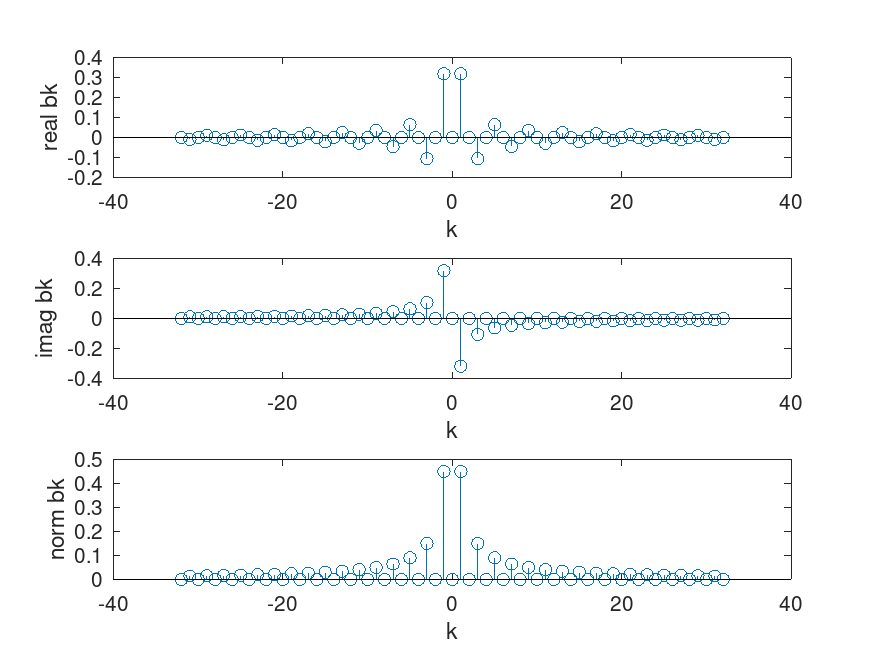
\includegraphics[width=0.7\linewidth]{code/dominio_frecuencia_delta}
	\caption{Dominio de la frecuencia ejemplo \ref{tren.de.pulsos.suma}}
	\label{fig:dominiofrecuenciadelta}
\end{figure}

\begin{figure}
	\centering
	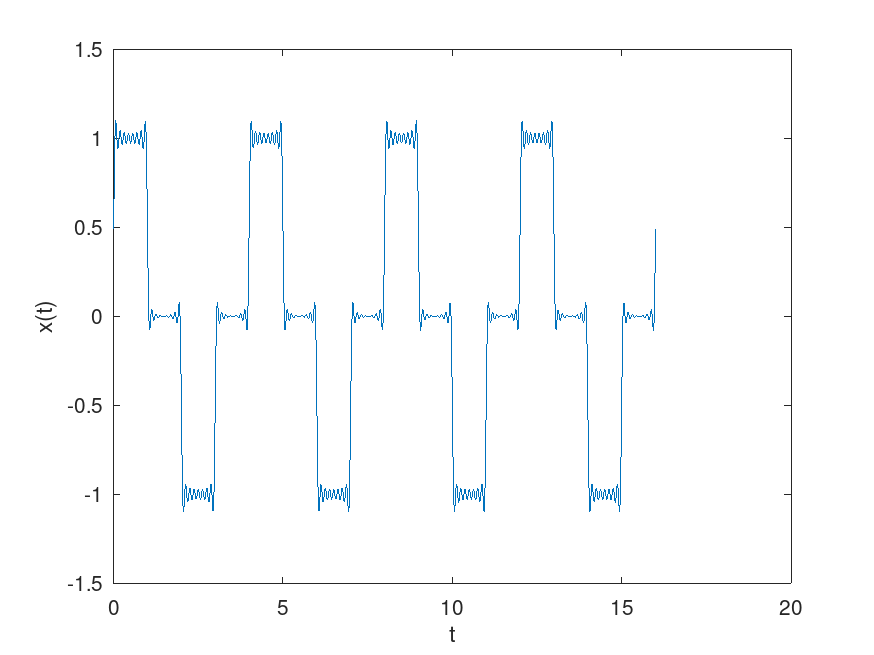
\includegraphics[width=0.7\linewidth]{code/dominio_tiempo_delta}
	\caption{Dominio del tiempo ejemplo \ref{tren.de.pulsos.suma}}
	\label{fig:dominiotiempodelta}
\end{figure}

\subsection{Una función periódica par \label{funcion.par}}

\begin{enumerate}
\item  Calculemos la serie de Fourier de la se\~{n}al definida por
\begin{equation}
x_{4}\left( t\right) = x_{4}(t+2 \, T)\left\{ 
\begin{array}{cc}
0   & -T < t \leq -T_{1}, \\
1  & -T_{1} < t \leq T_{1}, \\ 
0  & T_{1} < t \leq T.
\end{array}
\right. \label{squarewaveone.1}
\end{equation}
\item La ecuación de análisis (\ref{anafs}) para este caso es
\begin{equation}
2 \, T \, a_{k} = 
\int_{-T_{1}}^{T_{1}} e^{-j \, k \,\frac{2 \, \pi }{2 \, T} \, t} \, dt.
\end{equation}
\item Para $k = 0$,
\begin{equation}
2 \, T \, a_{0} = 
\int_{-T_{1}}^{T_{1}} e^{-j \, 0 \,\frac{2 \, \pi }{2 \, T} \, t} \, dt = 2 \, T_{1}.
\end{equation}
\begin{equation}
a_{0} = \frac{2 \, T_{1}}{2 \, T} = \frac{T_{1}}{T}.
\end{equation}
\item Para $k \neq 0$,
\begin{equation}
2 \, T \, a_{k} = 
\frac{\int_{-T_{1}}^{T_{1}} e^{-j \, k \,\frac{\pi }{T} \, t} \, d(-j \, k \,\frac{\pi }{T})t}{-j \, k \,\frac{\pi }{T}}.
\end{equation}
\item Evaluamos la integral
\begin{equation}
2 \, T \, a_{k} = 
\frac{\left[e^{\frac{-j \, k \, \pi \, t}{T}}\right]_{-T_{1}}^{T_{1}}}{\frac{j \, k \, \pi }{T}} =
\frac{e^{\frac{-j \, k \, \pi \, T_{1}}{T}}-
	  e^{\frac{j \, k \, \pi \, T_{1}}{T}}}{\frac{-j \, k \, \pi }{T}}.
\end{equation}
\item Simplificamos expresiones
\begin{equation}
a_{k} = \frac{e^{\frac{-j \, k \, \pi \, T_{1}}{T}}-
	e^{\frac{j \, k \, \pi \, T_{1}}{T}}}{-2 \, j \, k \, \pi} = 
    \frac{e^{\frac{j \, k \, \pi \, T_{1}}{T}}-
	e^{\frac{-j \, k \, \pi \, T_{1}}{T}}}{2 \, j \, k \, \pi} = 
    \frac{sin(\frac{k \, \pi \, T_{1}}{T})}{k \, \pi}
.
\end{equation}
\item Multiplicando y dividiendo
\begin{equation}
	a_{k} =  \frac{T_{1}}{T} \, \frac{sin(\frac{k \, \pi \, T_{1}}{T})}{k \, \pi \, \frac{T_{1}}{T}}
	.
\end{equation}
\item
Resumiendo
\begin{equation}
 a_{0} = \frac{T_{1}}{T_{2}},
\end{equation}
y
\begin{equation}
	a_{k} =  \frac{T_{1}}{T} \, \frac{sin(\frac{k \, \pi \, T_{1}}{T})}{k \, \pi \, \frac{T_{1}}{T}}
.
\end{equation}

\end{enumerate}

\lstinputlisting[language=Octave]{./code/echo.m}

\begin{figure}
	\centering
	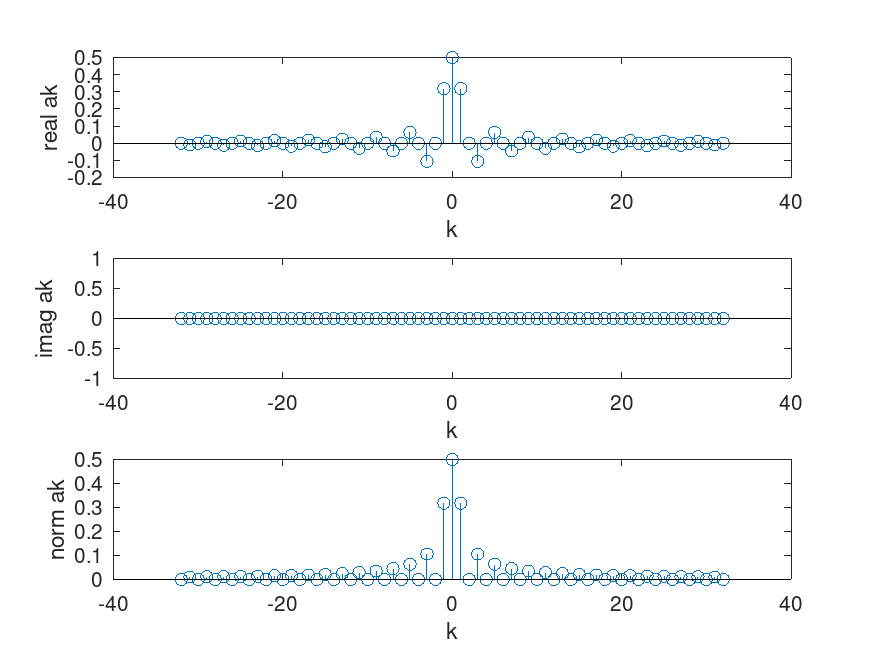
\includegraphics[width=0.7\linewidth]{code/dominio_frecuencia_echo}
	\caption{Dominio de la frecuencia ejemplo \ref{funcion.par}}
	\label{fig:dominiofrecuenciaecho}
\end{figure}

\begin{figure}
	\centering
	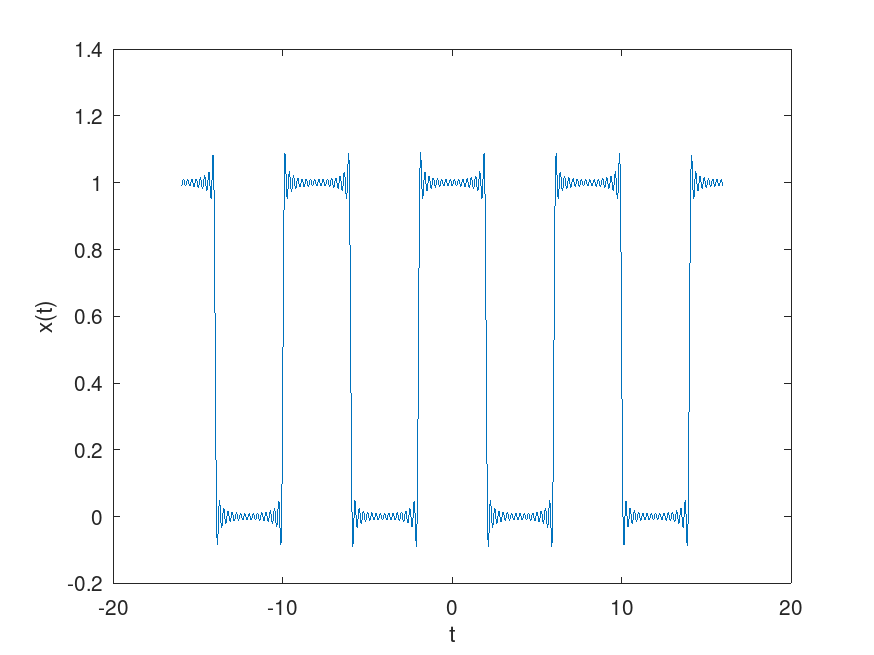
\includegraphics[width=0.7\linewidth]{code/dominio_tiempo_echo}
	\caption{Dominio del tiempo ejemplo \ref{funcion.par}}
	\label{fig:dominiotiempoecho}
\end{figure}

\subsection{Una función periódica impar \label{funcion.impar}}

\begin{enumerate}
	\item  Calculemos la serie de Fourier de la se\~{n}al definida por
	\begin{equation}
		x_{5}\left( t\right) = x_{4}(t+2 \, T)\left\{ 
		\begin{array}{cc}
			0   & -T < t \leq -T_{1}, \\
			-1  & -T_{1} < t \leq 0, \\ 
			1   & 0 < t \leq T_{1}, \\
			0  & T_{1} < t \leq T.
		\end{array}
		\right. \label{squarewavetwo.1}
	\end{equation}
	\item La ecuación de análisis (\ref{anafs}) para $k = 0$ es
    \begin{equation}
	2 \, T \, a_{0} = 
	-\left(\int_{-T_{1}}^{0}  \, dt\right)
	+\left(\int_{0}^{T_{1}}  \, dt\right)	= 0.
    \end{equation}

	\item La ecuación de análisis (\ref{anafs}) para $k \neq 0$ es
	\begin{equation}
		2 \, T \, a_{k} = 
		-\left(\int_{-T_{1}}^{0} e^{-j \, k \,\frac{2 \, \pi }{2 \, T} \, t} \, dt\right)
		+\left(\int_{0}^{T_{1}} e^{-j \, k \,\frac{2 \, \pi }{2 \, T} \, t} \, dt\right).
		\label{squarewavetwo.2}
	\end{equation}

	\item Para resolver (\ref{squarewavetwo.2}) multiplicamos y dividimos por $-j \, k \, \frac{\pi}{T}$
\begin{equation}
	2 \, T \, a_{k} = 
	-\frac{\left[e^{-j \, k \,\frac{\pi }{T} \, t} \right]_{-T_{1}}^{0}}{-j \, k \, \frac{\pi}{T}} 
	+\frac{\left[e^{-j \, k \,\frac{\pi }{T} \, t} \right]_{0}^{T_{1}}}{-j \, k \, \frac{\pi}{T}}.
	\label{squarewavetwo.3}
\end{equation}

	\item Escribamos
\begin{equation}
	-j \, 2 \, T \, k \, \frac{\pi}{T} \, a_{k} = 
	-\left[e^{-j \, k \,\frac{\pi }{T} \, t} \right]_{-T_{1}}^{0} 
	+\left[e^{-j \, k \,\frac{\pi }{T} \, t} \right]_{0}^{T_{1}}.
	\label{squarewavetwo.4}
\end{equation}

\item 
\begin{equation}
	-j \, 2 \, k \, \pi \, a_{k} = 
-\left(1 - e^{j \, k \,\frac{\pi }{T} \, T_{1}} \right) 
+\left(e^{-j \, k \,\frac{\pi }{T} \, T_{1}} - 1 \right).
	\label{squarewavetwo.5}
\end{equation}
\item 
\begin{equation}
	-j \, 2 \, k \, \pi \, a_{k} = 
	e^{j \, k \,\frac{\pi }{T} \, T_{1}}
	+e^{-j \, k \,\frac{\pi }{T} \, T_{1}} - 2.
	\label{squarewavetwo.6}
\end{equation}
\item 
\begin{equation}
	-j \, 2 \, k \, \pi \, a_{k} = 
	e^{j \, k \,\frac{\pi }{T} \, T_{1}}
	+e^{-j \, k \,\frac{\pi }{T} \, T_{1}} - 2.
	\label{squarewavetwo.7}
\end{equation}
\item 
\begin{equation}
	a_{k} = 
	\frac{2 - e^{j \, k \,\frac{\pi }{T} \, T_{1}}
	-e^{-j \, k \,\frac{\pi }{T} \, T_{1}}}{j \, 2 \, k \, \pi \,}.
	\label{squarewavetwo.8}
\end{equation}
\item 
\begin{equation}
	a_{k} = \frac{T_{1}}{T} \,
	\frac{1 - cos(k \,\frac{\pi }{T} \, T_{1})}{
	j \, k \, \pi \, \frac{T_{1}}{T}}.
	\label{squarewavetwo.9}
\end{equation}
\end{enumerate}

\lstinputlisting[language=Octave]{./code/foxtrot.m}

\begin{figure}
	\centering
	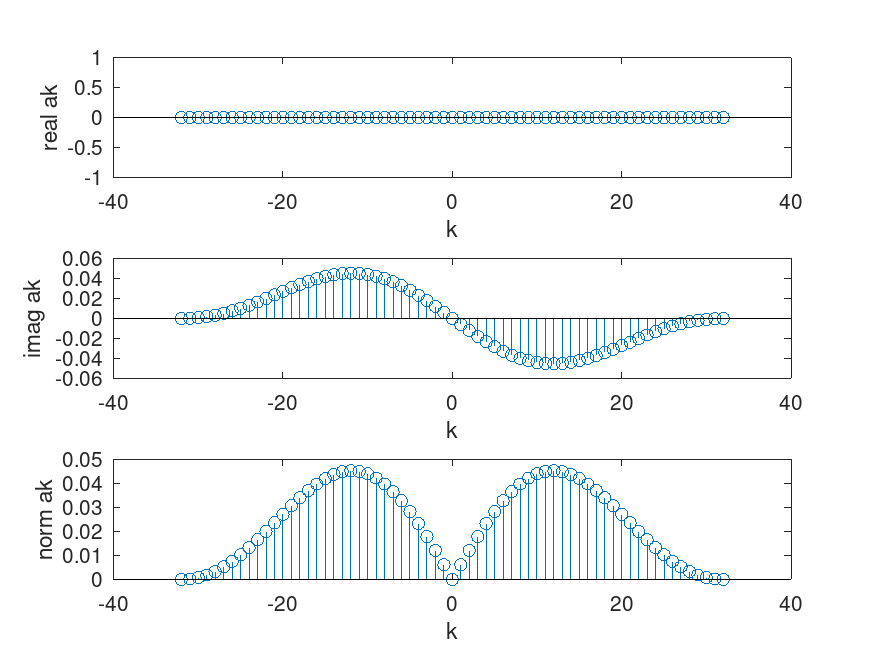
\includegraphics[width=0.7\linewidth]{code/dominio_frecuencia_foxtrot}
	\caption{Dominio de la frecuencia ejemplo \ref{funcion.impar}}
	\label{fig:dominiofrecuenciafoxtrot}
\end{figure}

\begin{figure}
	\centering
	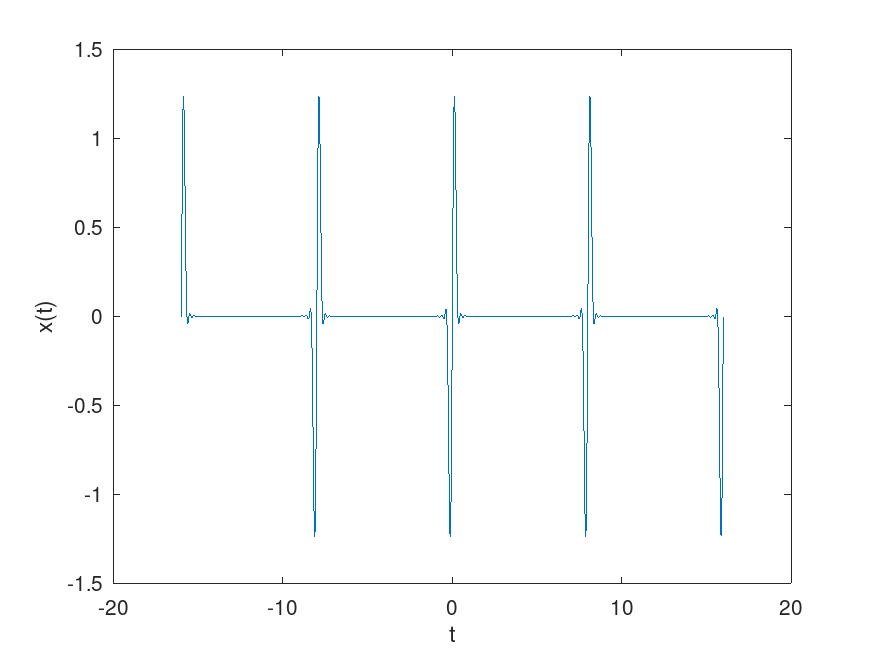
\includegraphics[width=0.7\linewidth]{code/dominio_tiempo_foxtrot}
	\caption{Dominio del tiempo ejemplo \ref{funcion.impar}}
	\label{fig:dominiotiempofoxtrot}
\end{figure}

\section{Sistema lineal excitado con una serie de Fourier}

\begin{enumerate}
\item Supongamos que tenemos un sistema lineal invariante en el tiempo con una respuesta al impulso $h(t)$. Vamos a calcular la salida $y(t)$ para una entrada
\begin{equation}
	x(t) = \sum_{k=-\infty}^{\infty} a_{k} \, e^{j \, k \, \frac{2 \, \pi}{T} \, t}. 
	\label{conv.tc.seriedefourier.alpha}
\end{equation}

\item Para evaluar la integral de convolución, emplearemos la fórmula
\begin{equation}
	y(t) = \int_{-\infty}^{\infty} h(v) \, x(t - v) \, dv. 
	\label{conv.tc.seriedefourier.bravo}	
\end{equation}

\item Reemplazando (\ref{conv.tc.seriedefourier.alpha}) en (\ref{conv.tc.seriedefourier.bravo}) obtenemos
\begin{equation}
	y(t) = \int_{-\infty}^{\infty} h(v) \, \left(
	\sum_{k=-\infty}^{\infty} a_{k} \, e^{j \, k \, \frac{2 \, \pi}{T} \, (t-v)}
	\right)
	dv. 
	\label{conv.tc.seriedefourier.charlie}	
\end{equation}
\item Intercambiamos la posición del signo de integral con el signo de sumatoria
y factoreamos la exponencial
\begin{equation}
	y(t) = \sum_{k=-\infty}^{\infty} 
	\int_{-\infty}^{\infty} h(v) \, 
	 a_{k} \, e^{j \, k \, \frac{2 \, \pi}{T} \, t} \, e^{-j \, k \, \frac{2 \, \pi}{T} \, v}
	dv. 
	\label{conv.tc.seriedefourier.delta}	
\end{equation}
\item Podemos extraer el factor $a_{k} \, e^{j \, k \, \frac{2 \, \pi}{T} \, t}$ fuera de las integrales en (\ref{conv.tc.seriedefourier.delta})
\begin{equation}
	y(t) = \sum_{k=-\infty}^{\infty} 
	\left(\int_{-\infty}^{\infty} h(v) \, 
	 \, e^{-j \, k \, \frac{2 \, \pi}{T} \, v}
	dv\right) \, a_{k} \, e^{j \, k \, \frac{2 \, \pi}{T} \, t}.
	\label{conv.tc.seriedefourier.echo}	
\end{equation}
\item En la ecuación (\ref{conv.tc.seriedefourier.echo}) podemos definir
\begin{equation}
	H(k \, \frac{2 \, \pi}{T}) = \int_{-\infty}^{\infty} h(v) \, 
	\, e^{-j \, k \, \frac{2 \, \pi}{T} \, v}
	dv,
\end{equation}
y escribir
\begin{equation}
	y(t) = \sum_{k=-\infty}^{\infty} 
	 H(j \, k \, \frac{2 \, \pi}{T}) \, a_{k} \, e^{j \, k \, \frac{2 \, \pi}{T} \, t}.
	\label{conv.tc.seriedefourier.foxtrot}	
\end{equation}

\item Los factores $H(j \, k \, \frac{2 \, \pi}{T})$ son evaluaciones de la transformada de Fourier $H(j \, \omega)$ para los valores de frecuencia $j \, k \, \frac{2 \, \pi}{T}$. Si elegimos los valores de $H(j \, k \, \frac{2 \, \pi}{T})$ en forma adecuada, podemos procesar la señal de entrada para obtener una salida conveniente o adecuada. Esto es el principio matemático de los filtros de señal.

\end{enumerate}
%\section{Modulación}
%
%¿Qué pasa cuando multiplicamos dos funciones periódicas?
%
%\subsection{El caso más sencillo}
%
%Consideremos la multiplicación de dos señales períodicas con períodos que no son necesariamente iguales
%\begin{equation}
% x_{1}(t) = e^{j \, \frac{2 \, \pi}{T_{1}} \, t},
%\end{equation}
%\begin{equation}
% x_{2}(t) = e^{j \, \frac{2 \, \pi}{T_{2}} \, t},
%\end{equation}
%y
%\begin{equation}
% y(t) = x_{1}(t) \, x_{2}(t) = e^{j \, \frac{2 \, \pi}{T_{1}} \, t} \, e^{j \, \frac{2 \, \pi}{T_{2}} \, t}.
%\end{equation}
%La pregunta es ¿Cuál es el período $T$ de $y(t)$?
%Si hacemos
%\begin{equation}
% y(t) = e^{j \, \frac{2 \, \pi}{T_{1}} \, t} \, e^{j \, \frac{2 \, \pi}{T_{2}} \, t} = 
% e^{j \, \left(\frac{1}{T_{1}} + \frac{1}{T_{2}}\right) \, 2 \, \pi \, t},
%\end{equation}
%que debe ser
%\begin{equation}
% y(t) = e^{j \, \frac{2 \, \pi}{T} \, t} =
% e^{j \, \left(\frac{1}{T_{1}} + \frac{1}{T_{2}}\right) \, 2 \, \pi \, t}.
%\end{equation}
%Por lo tanto resulta
%\begin{equation}
% \frac{1}{T} = \frac{1}{T_{1}} + \frac{1}{T_{2}}.
%\end{equation}
%
%\subsection{Una serie de Fourier con $M$ armónicas multiplicada por una exponencial imaginaria}
%
%Consideremos ahora el caso de una serie de Fourier
%\begin{equation}
% x_{1}(t) = \sum_{k=-M}^{M} a_{k} \, e^{j \, k \, \frac{2 \, \pi}{T_{1}} \, t},
%\end{equation}
%y el producto
%\begin{equation}
% y(t) =  \left(
% \sum_{k=-M}^{M} a_{k} \, e^{j \, k \, \frac{2 \, \pi}{T_{1}} \, t}
% \right) \, e^{j \, \frac{2 \, \pi}{T_{2}} \, t}.
%\end{equation}
%Por la propiedad distributiva del producto respecto a la suma
%\begin{equation}
% y(t) =  
% \sum_{k=-M}^{M} a_{k} \, e^{j \, (k \, \frac{2 \, \pi}{T_{1}} +  \frac{2 \, \pi}{T_{2}})\, t}
%,
%\end{equation}
%podemos escribir
%\begin{equation}
% y(t) =  
% \sum_{k=-M}^{M} a_{k} \, e^{j \, (\frac{k}{T_{1}} +  \frac{1}{T_{2}})\, 2 \, \pi \, t}
%.
%\end{equation}
%Observe que en esta ecuación, no tenemos una serie de Fourier propiamente dicha porque en
%\begin{equation}
%	\frac{k}{T_{1}} +  \frac{1}{T_{2}} \neq \frac{p}{Q \, T},
%\end{equation}
%no tenemos una expresión de donde obtener $T$ para $Q \in N$, $p \in N$.
%
%\subsection{Una serie de Fourier con $M$ armónicas multiplicada por una función cos}
%
%Considerando
%\begin{equation}
%	p(t) =  \left(
%	\sum_{k=-M}^{M} a_{k} \, e^{j \, k \, \frac{2 \, \pi}{T_{1}} \, t}
%	\right) \, e^{j \, \frac{2 \, \pi}{T_{2}} \, t}, 
%\end{equation}
%y
%\begin{equation}
%	q(t) =  \left(
%	\sum_{k=-M}^{M} a_{k} \, e^{j \, k \, \frac{2 \, \pi}{T_{1}} \, t}
%	\right) \, e^{-j \, \frac{2 \, \pi}{T_{2}} \, t}, 
%\end{equation}
%podemos escribir
%\begin{equation}
%	r(t) = p(t) + q(t) =
%	\left( 
%	\sum_{k=-M}^{M} a_{k} \, e^{j \, k \, \frac{2 \, \pi}{T_{1}} \, t} \, e^{j \, \frac{2 \, \pi}{T_{2}} \, t} 	
%	\right) +
%	\left( 
%    \sum_{k=-M}^{M} a_{k} \, e^{j \, k \, \frac{2 \, \pi}{T_{1}} \, t} \, e^{-j \, \frac{2 \, \pi}{T_{2}} \, t} 	
%    \right).
%\end{equation}
%\begin{equation}
%	r(t) = p(t) + q(t) =
%	\sum_{k=-M}^{M} a_{k} \, 	\left( e^{j \, \left(\frac{k}{T_{1}} + \frac{1}{T_{2}}\right) \, 2 \, \pi \, t} + e^{j \, \left(\frac{k}{T_{1}} - \frac{1}{T_{2}}\right) \, 2 \, \pi \, t}
%	\right).
%\end{equation}

\section{Ejercicios}

% Signals and Systems with Matlab 2009, pages 65 - 67

\begin{enumerate}
\item Obtenga coeficientes de Fourier (para una serie expresada como suma ponderada de exponenciales imaginarias) 
para una se\~{n}al triangular obtenida integrando la se\~{n}al $x_{5}(t)$ definida arriba en la ecuaci\'{o}n (\ref{squarewave}). 
Grafique el espectro correspondiente.

\item Obtenga coeficientes de Fourier (para una serie expresada como suma ponderada de exponenciales imaginarias) 
para una se\~{n}al triangular obtenida integrando la se\~{n}al $x_{6}(t)$ definida arriba en la ecuaci\'{o}n (\ref{squarewaveone.1}). 
Grafique el espectro correspondiente.

\item Obtenga coeficientes de Fourier (para una serie expresada como suma ponderada de exponenciales imaginarias) 
para la se\~{n}al per\'{o}dica $T$, tal que $0 < T_{1} \leq T$, definida como
\begin{equation}
x_{7}(t) = \left\{\begin{array}{cc}
  1 & |t - k \, T| \leq \frac{T_{1}}{2}, \\
    & \\
  0 & |t - k \, T| > \frac{T_{1}}{2},
\end{array} \right.
\end{equation}
Compruebe que los coeficientes se pueden definir como
\begin{equation}
c_{k} = T_{1} \, \frac{sin(k \, \frac{2 \, \pi}{T} \frac{T_{1}}{2})}{k \, \frac{2 \, \pi}{T} \frac{T_{1}}{2}}.
\end{equation}
Explique que sucede cuando $k = 0$.
\item Desplaze la se\~{n}al $x_{5}$ en el tiempo hasta que coincida con la se\~{n}al $x_{7}$. \textquestiondown Que factor es el necesario para modificar los coeficientes de $x_{5}$ para que coincidan con los de $x_{7}$?
\end{enumerate}

